\subsubsection{System Topologie}
\begin{figure}[H]
\centering
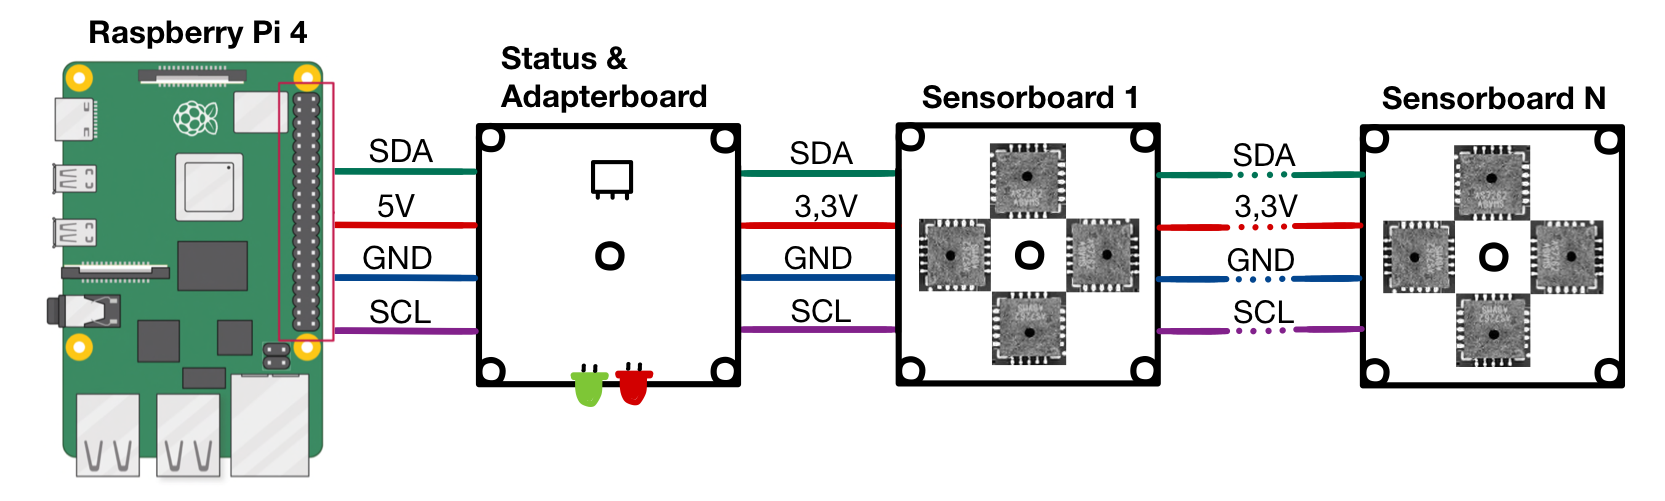
\includegraphics[width=1\textwidth]{img/System-Topologie.png}
%\caption*{Quelle: Datenblatt AS7261}
\caption{Verschaltung der der Platienen}
\label{fig:Seitenasicht-AS726X}
\end{figure}

Der Msssaufbau besteht aus einem Rapberry Pi 4 Model B welcher über eine status und Adapterplatinene mit 1-10 Sensnorboards verbunden werden kann.


\subsubsection{Status \& Adapterboard}
Da der Rapberry Pi nicht die benötigte $3,3V$ Stromversorgung bereitstellt wird eine Adapter-Shield mit einem Spannungswandler(LM3940IT-3.3) verwendet.
Auf dem Adapter-Shield findet der einheitliche Steckverbinder sowie die Pull Up widerstände des I2C Bus Platz, da das Adapter-Shield aufgrund seiner Bauform nicht falsch montiert werden kann so die Verpolung der Sensoren ausgeschlossen werden.
Die Bedeutung der Status LED wird im Handbuch \ref{todo} erläutert.\\
Der überflüssige Platz auf dem Adapter-Shield wurde für einen Prototyping-Bereich genutzt.

\begin{figure}[H]
\centering
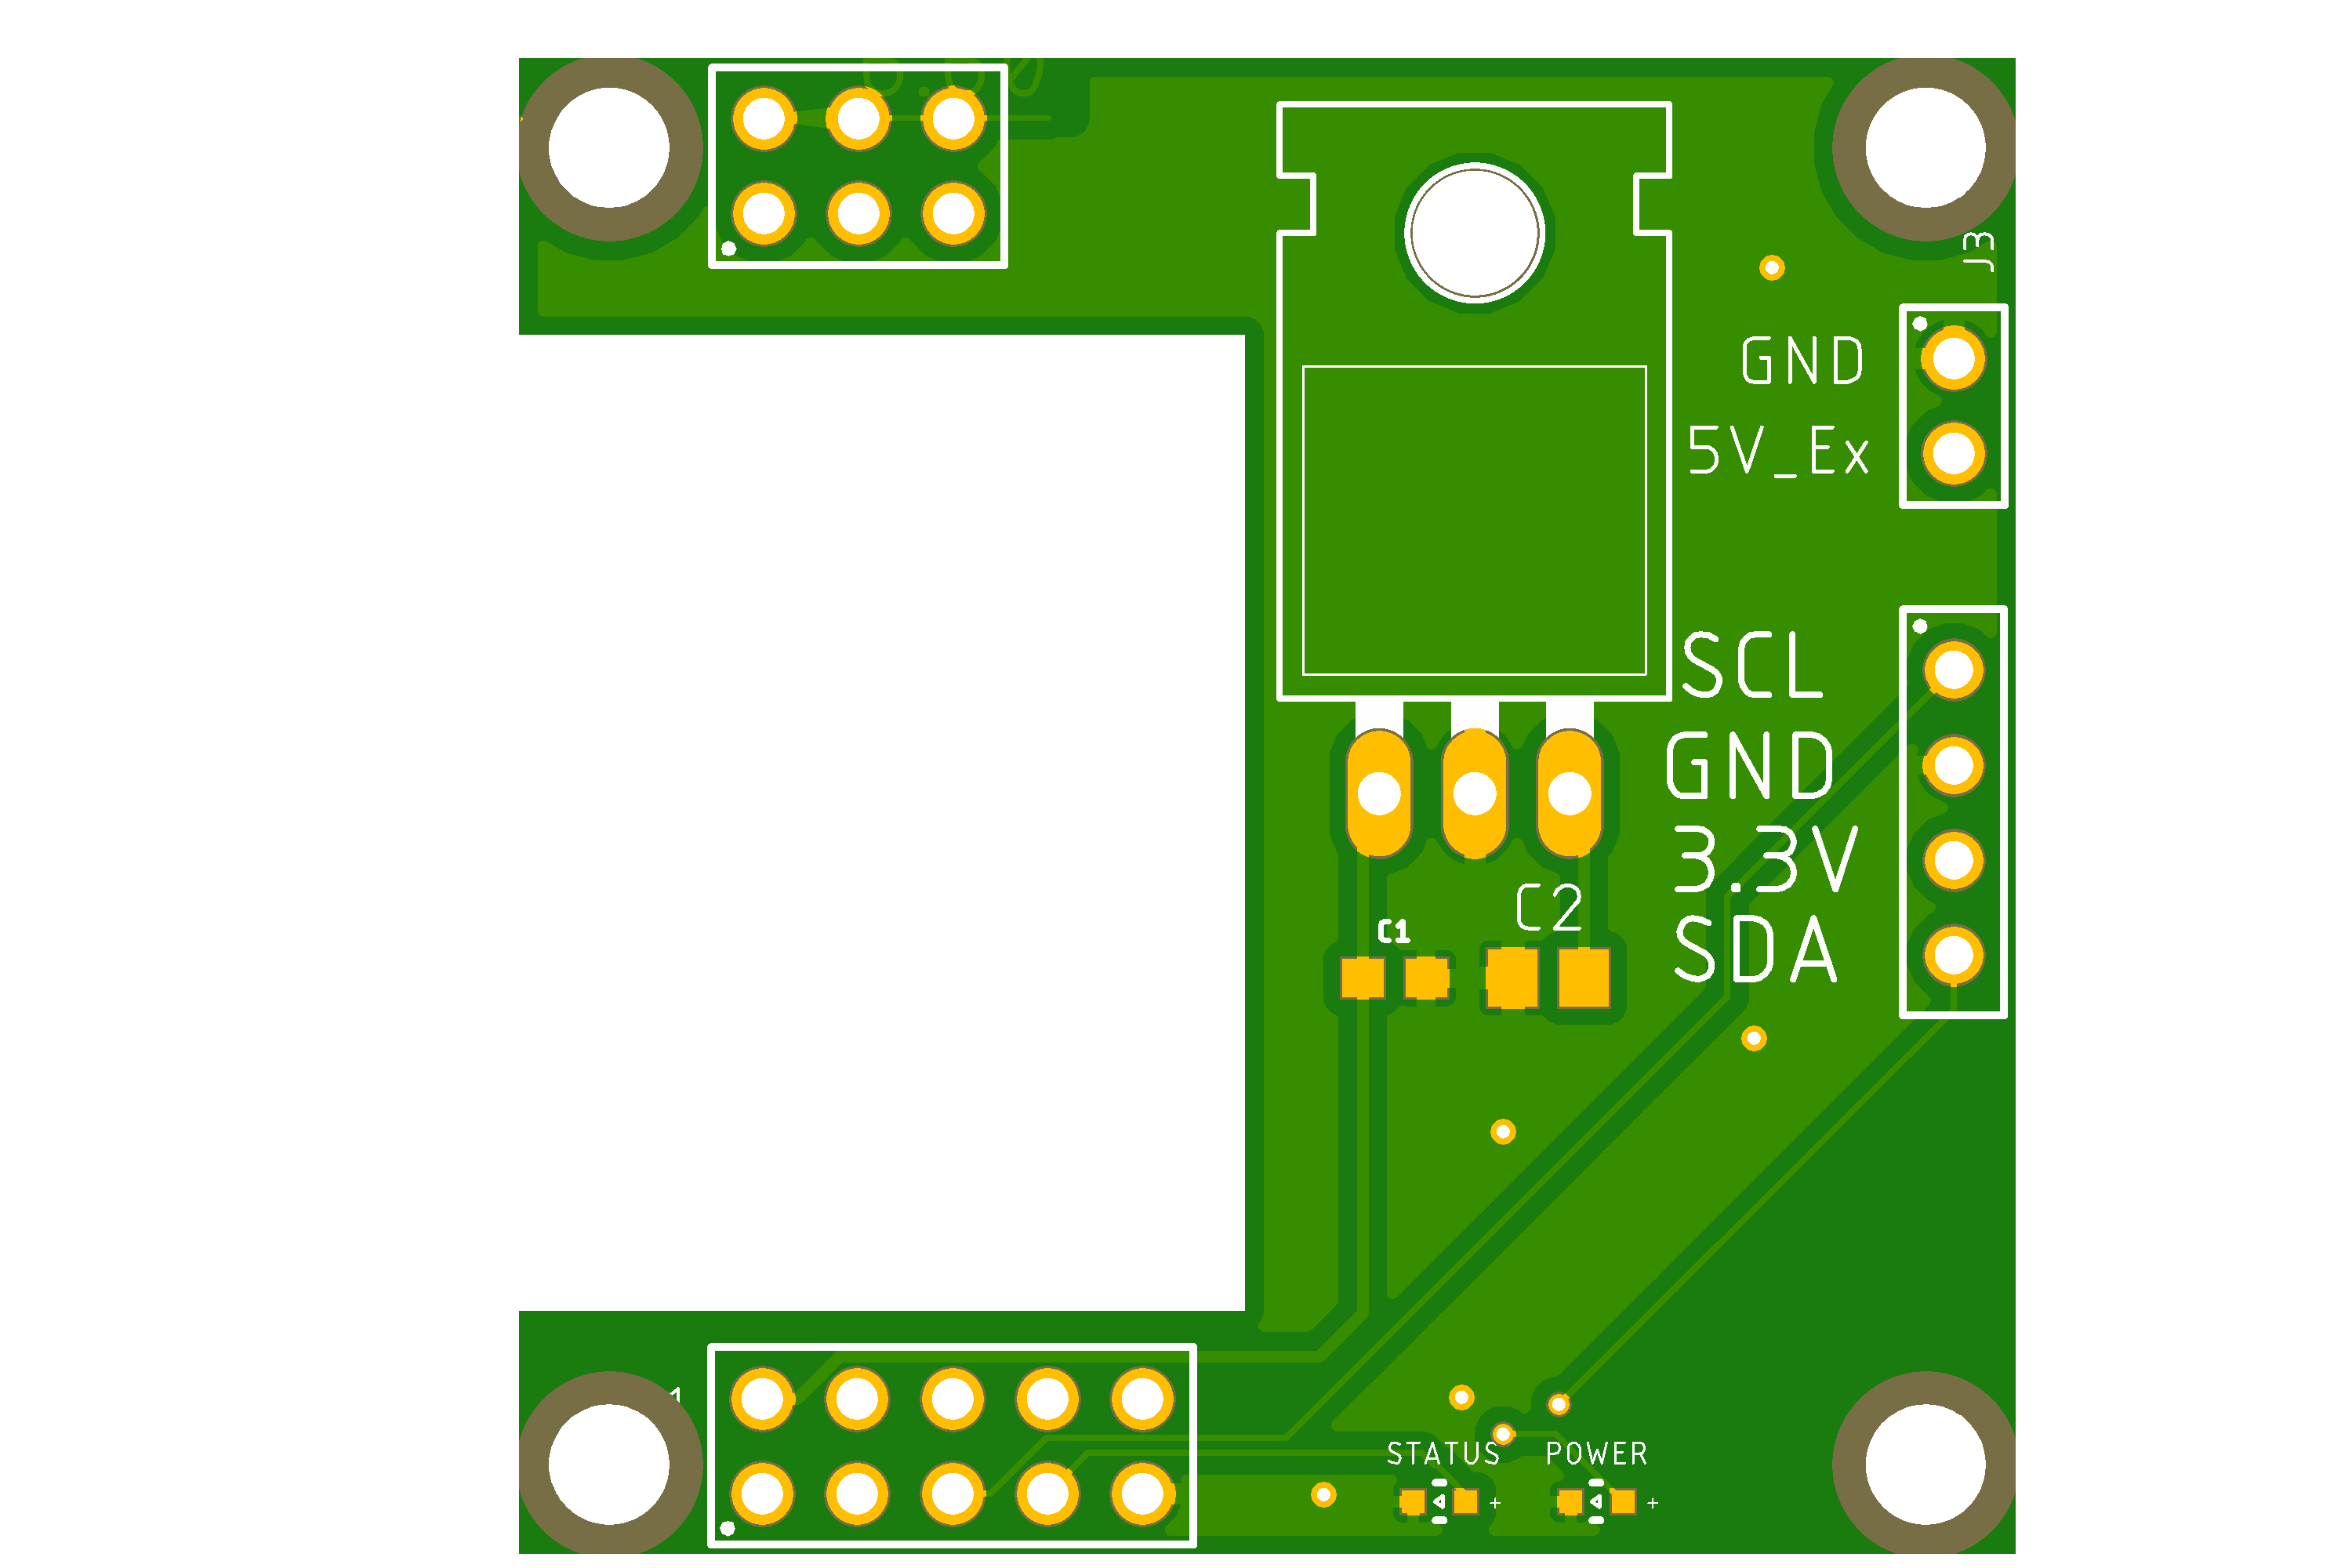
\includegraphics[width=0.75\textwidth]{img/nanopi-black2-shield}
%\caption*{Quelle: Datenblatt AS7261}
\caption{Verschaltung der der Platienen}
\label{fig:Seitenasicht-AS726X}
\end{figure}
\subsubsection{Sensorboard}
Die hauptaufgabe der Sensorboard Platine ist es den AS7261 und der AS7265X mit ihrem companion flash (\ref{Todo}) und über den I2C Translator (\ref{TODO}) dem I2C Bus verbunden.
Außerdem werden verschiednene LED, Wiederstände und Kondensatoren verbaut.

\begin{figure}[H]
\centering
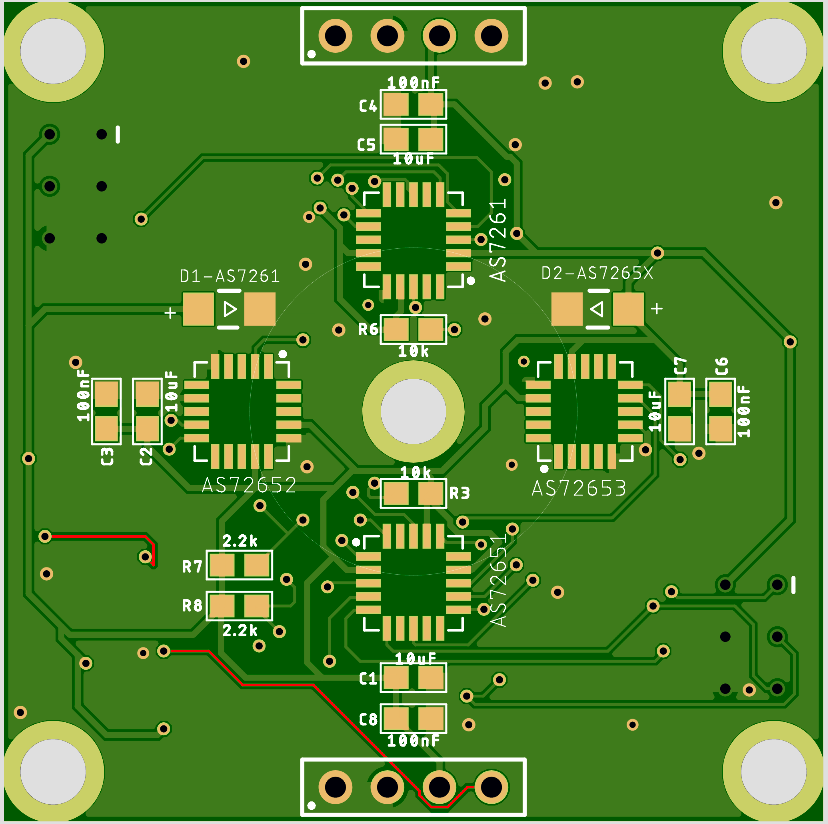
\includegraphics[width=0.75\textwidth]{img/Sensor-platiene_front}
%\caption*{Quelle: Datenblatt AS7261}
\caption{Verschaltung der der Platienen}
\label{fig:Seitenasicht-AS726X}
\end{figure}

\begin{figure}[H]
\centering
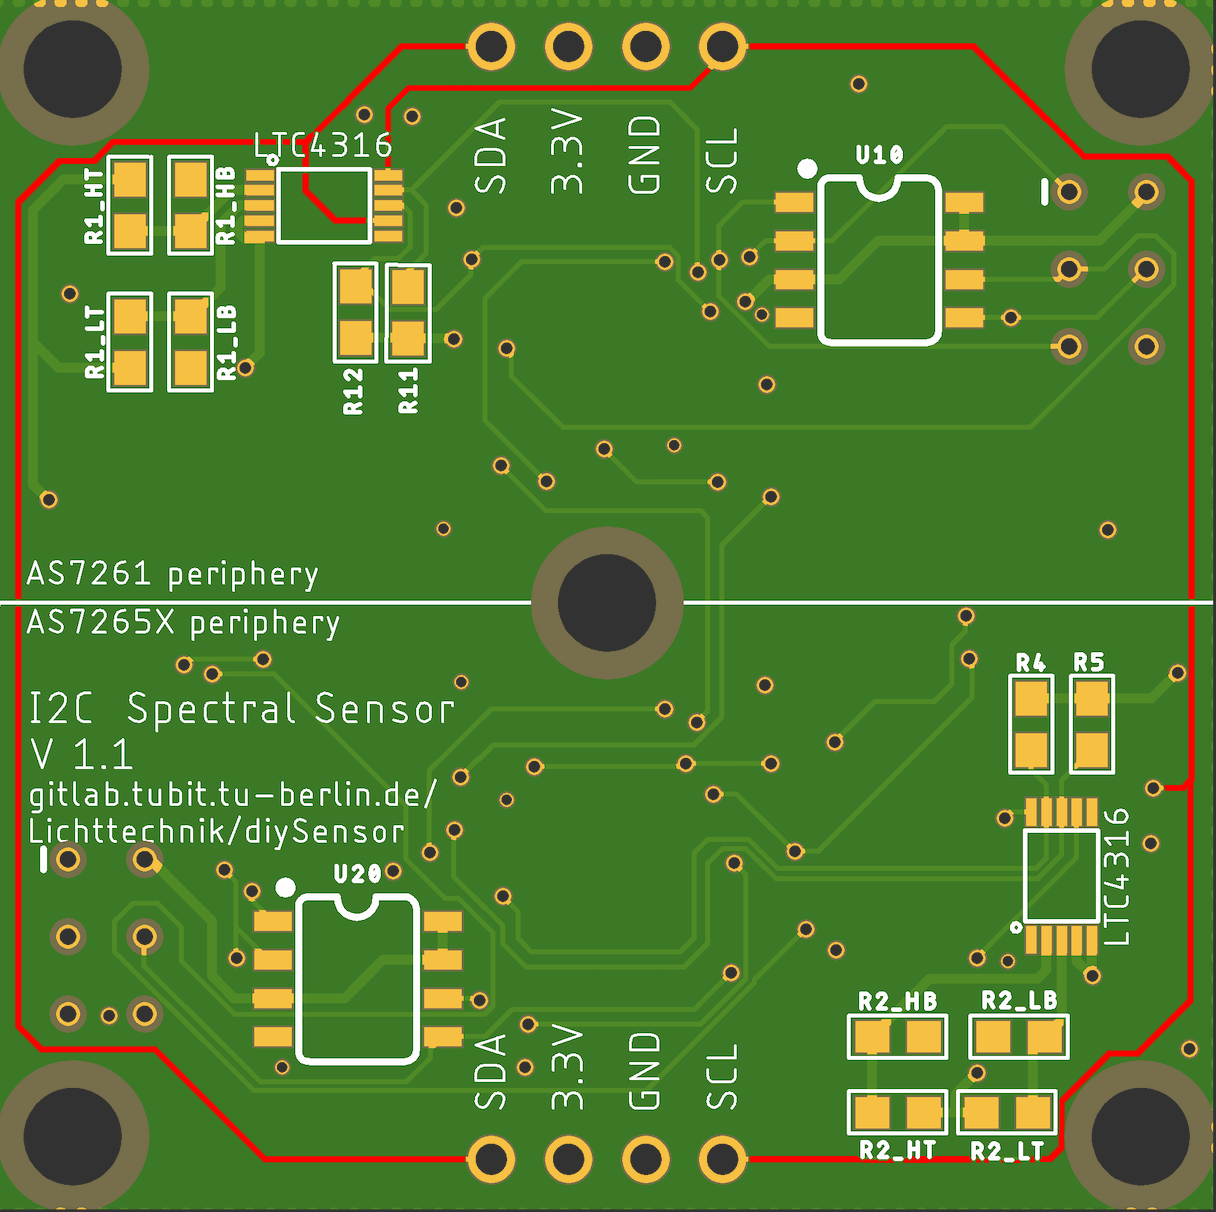
\includegraphics[width=0.75\textwidth]{img/Sensor-platiene_back}
%\caption*{Quelle: Datenblatt AS7261}
\caption{Verschaltung der der Platienen}
\label{fig:Seitenasicht-AS726X}
\end{figure}

\paragraph{Status LED:} Am AS7261 und AS7265X Befindet sich jewals eine Rote Status LED wenn es ein problem mit dem Compainin Flash gibt fängt sie an zu blinken im normalbetrieb kann die LED Softwareseitg ein und ausgeschaltet werden.
	Wärend der Messubng solle sie ausgeschaltet werden da das Rote licht sonst die Messung verfälscht.

\paragraph{Pull-up-Widerstände:}
R7 und R8 sind die Pullup Widerstände des seperaten I2C Bus welcher die AS7265X Sensoren miteinander verbindet.\\
R12 und R11 sind die Pullup Widerstände des I2C Bus welcher den AS7261 mit seinem LCT4316 verbindet.\\
R4 und R5 sind die Pullup Widerstände des I2C Bus welcher den AS72651 mit seinem LCT4316 verbindet.

\paragraph{I2C Enable Wiederstände:} Pin R6 ist mit 3.3V und Pin 8 (I2C Enable) des AS7261 verbunden. So wird der AS7261 in den I2C modus gebracht.
	R3 erfüllt die gleiche Aufgabe für den AS72651.
	
\paragraph{Translation Byte Wiederstände:}
Die 8 Wiederstände auf der Rückseite R1\_XX und R2\_XX sind die in \ref{TODO} beschriebenen wiederstände welche das Translation Byte einstellen. Die wiederstände R1\_XX bestimmen die Addresse des AS7261 und R1\_XX die Addresse des AS72651.

\paragraph{Entstörkondensatoren:} Das Datenblatt der Sensoren emphielt für jeden Sensor 2 Entstörkondensatoren möglichst nah am Sensor zwischen GND und VCC anzubringen.


\begin{center}
\begin{tabular}{ c c c }
 Kürzel & Wert & Sensor \\ 
 C5 & $10uF$ & AS7261 \\  
 C4 & $100nF$ & AS7261 \\
 C1 & $10uF$ & AS72651 \\  
 C8 & $100nF$ & AS72651 \\
 C2 & $10uF$ & AS72652 \\  
 C3 & $100nF$ & AS72652 \\
 C7 & $10uF$ & AS72653 \\  
 C6 & $100nF$ & AS72653 \\
\end{tabular}
\end{center}


\paragraph{I2C Lanes:}
Die I2C Leitungen haben ihren Ursprung auf der Adapterplatine und werden mithilfe der seitlichen Steckverbinder über die Sensnsorboards durchgeschleift.
Die maximal mögliche länge einer I2C Leitung hängt von der länge der Leitungskapazität sowie äußeren Störeinflüssen ab.
Die Data und die Clock Leitung sind möglichst weit von anderen Datenleitungen  also auch von einander entfernt platziert, da so Störeinflüsse durch elektromagnetische Felder minimiert werden.
Außerdem wurde darauf geachtet das die Leitungen auf den Platinen die gleiche länge habe da sich sonst die Differenzen der Leitungslänge mit jeder angeschlossenen Platine addiert und es zu Timing Differenzen zwischen der Daten und Clock Leitung kommt.
Der Verlauf der Leitungen ist in Abb\ref{Todo} Rot gekennzeichnet.

\paragraph{Connector:} An Rechts und Links an der Platine befinden sich 4 durchkontaktierte Löcher, hier können unterschiedliche Steckverbinder mit 2.54 mm Pitch montiert werden.
	Es empfiehlt sich, verpolungssichere Steckverbinder zu verwenden, um Hardware Schäden vorzubeugen.
	Für dieses Bauteil wurde keine SMD-Technik, sonder Durchsteckmontage gewählt, da so eine bessere mechanische Festigkeit erreicht wird.
	Außerdem kann so alternativ zu einem Steckverbinder direkt ein Flachbandkabel angelötet werden.

